\chapter{Entropy, Types and the Rate Function of the Queens}
\label{ch:entropy}

The density of states\index{density of states} $N(s)$ is $e^{H(s)}$ for an entropy $H$, Simkin\index{Simkin's theorem}'s constant is an entropy, and the ladder length of the vertical walk is an entropy difference. This chapter gives the information theoretic view of the counting problem: the method of types, Sanov's theorem, the entropy chain rule as a counting tool, and the rate function for the number of attacking pairs in a random permutation, which we compute numerically from the exact density of states and conjecture as a variational problem over queenons.

\section{The method of types}

For a sequence of $n$ symbols from a finite alphabet, the type is the empirical distribution of symbols. There are at most $(n+1)^{|\mathcal{A}|}$ types, polynomially many, and the number of sequences of a given type $\nu$ is $\binom{n}{n \nu}$, which by Stirling is $e^{n H(\nu) + O(\log n)}$ where $H$ is the Shannon\index{Shannon, Claude} entropy. The probability of a type under an i.i.d. source $\mu$ is therefore $e^{-n D(\nu \| \mu) + O(\log n)}$, and Sanov's theorem states that the probability that the empirical distribution lies in a set $A$ is $e^{-n \inf_{\nu \in A} D(\nu \| \mu) + o(n)}$. Rare events are governed by the least improbable type that realises them, and the rate is a relative entropy.

Permutations are not i.i.d. sequences, but the method of types extends. A permutation of $[N]$ has a type in the sense of a block occupancy matrix on a $k \times k$ grid, normalised to sum to $1$, as in Simkin's proof, and the number of permutations with a given occupancy matrix $\nu$ is, by the asymptotics of the permanent\index{permanent} or by Stirling applied to the multinomial coefficients, $N! \, e^{-N D(\nu \| u_k) + o(N)}$ where $D(\nu \| u_k) = \sum_{ab} \nu_{ab} \log(k^2 \nu_{ab})$ is the relative entropy of $\nu$ from the uniform matrix $u_k$. The limiting objects as $k \to \infty$ are the doubly stochastic densities on the square, the permutons, and the queenon is a permuton.

\section{The entropy chain rule as a counting tool}

For a uniformly random solution $X = (x_1, \dots, x_N)$ the chain rule gives
\[
\log Q(N) = \sum_{i=1}^{N} H(x_i \mid x_1, \dots, x_{i-1}) ,
\]
and each term is at most the logarithm of the number of columns available to row $i$ given the earlier rows. This gives an upper bound on $Q(N)$ from any upper bound on the expected number of available columns, and it is the skeleton of Simkin's upper bound. In reverse, the vertical walk estimates each conditional entropy: the ratio $Z_{m_{t-1}} / Z_{m_t}$ is $e^{-\Delta H}$ for the entropy difference between consecutive level sets, and $\log \rho = \sum_t \log \theta_t$ is the total entropy drop from the uniform distribution on permutations to the uniform distribution on solutions. The ladder is a decomposition of an entropy into a sum of conditional entropies, each estimated by sampling, and the product estimator\index{product estimator}'s variance bound is a bound on how well a sum of $T$ conditional entropies can be estimated from $M$ samples each.

Shannon's source coding theorem gives this a concrete meaning. A uniformly random solution can be compressed to $\log_2 Q(N)$ bits and no fewer; a uniformly random permutation to $\log_2 N!$ bits; and the difference, $\log_2 (N! / Q(N))$, which is about $1.36 N$ bits by Simkin and the fit of Chapter~\ref{ch:open}, is the information that the constraint carries. The walk pays this many bits, in the form of rejected samples, to get from permutations to solutions, and $1.36 N$ bits at a ratio of one half per rung is $1.36 N$ rungs.

\section{The rate function of the attack count}

Let $S_N$ be the number of attacking pairs of a uniformly random permutation of $[N]$. Its mean is $2N/3 + O(1)$ by the calculation of Chapter~\ref{ch:phase}, and its distribution is concentrated: the variance is $O(N)$ by the pairwise structure, so the typical fluctuation is $O(\sqrt N)$. Large deviations ask for the probability that $S_N / N$ is near a value $e$ far from $2/3$, and the rate function is
\[
I(e) = -\lim_{N \to \infty} \frac{1}{N} \log \PP( S_N / N \approx e ) ,
\]
if the limit exists. Simkin's theorem gives $I(0) = \alpha - 1 = 0.942$. Nothing is proved about $I(e)$ for $e > 0$, and we offer a computation and a conjecture.

From the exact density of states for $N = 8$ to $11$, the function $-\log(N(s)/N!) / N$ against $s/N$ is plotted in Figure~\ref{fig:rate}. The curves for successive $N$ are close and converging to a convex curve with its minimum, zero, at $e \approx 0.65$ and value about $0.9$ at $e = 0$, with the finite size curves lying below the limit at $e = 0$ and rising towards it, as expected from the positive subexponential prefactor. The finite size minima sit at $e = 0.50$, $0.56$, $0.60$, $0.55$ for $N = 8$ to $11$, and the value $0.65$ is an extrapolation towards $2/3$. The curve rises steeply for $e$ above $1$, reflecting that configurations with many attacks are those near the main diagonals and are few.

\begin{figure}[t]
\centering
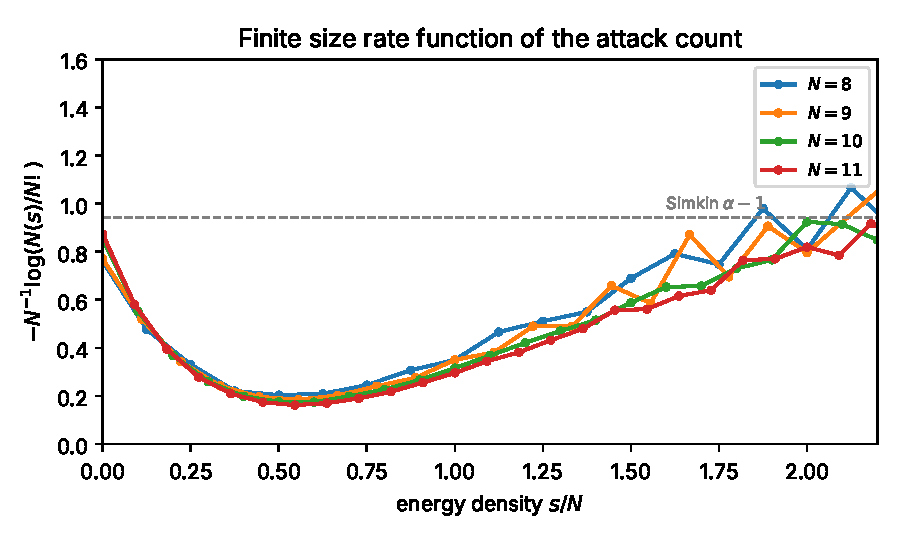
\includegraphics[width=0.85\textwidth]{fig_rate.pdf}
\caption{The finite size rate function $-N^{-1} \log(N(s)/N!)$ against the energy density $s/N$ for $N = 8$ to $11$, from the exact density of states. The curves converge to the large deviations rate function $I(e)$, with $I(0) = \alpha - 1 \approx 0.94$ by Simkin.}
\label{fig:rate}
\end{figure}

\begin{conjecture}
\label{conj:ratefn}
We conjecture that the rate function $I(e)$ exists, is convex on $[0, \infty)$ with $I(2/3) = 0$, and is given near $e = 0$ by a variational problem over queenon\index{queenon}like densities with prescribed attack density $e$ (queenons proper have $e = 0$): heuristically $I(e) = -\sup\{ \Psi(f) : f \text{ a queenon with attack density } e \}$ for the functional $\Psi$ of Simkin's upper bound (not the conductance of Chapter~\ref{ch:mixing}), suitably extended, so that $I(0) = \alpha - 1$. We do not prove this.
\end{conjecture}

The conjecture is the natural extension of Simkin's theorem from the ground state to every energy, and its proof would follow his method with the hard constraint of no attacks replaced by a soft constraint on the attack density. The payoff for the program is the staircase: the widths $N(s)/N!$ at energy $s = eN$ are $\exp(-N I(e) + o(N))$, and the vertical ladder's ratios are $\theta = \exp(-N (I(e - 1/N) - I(e))) \approx \exp(I'(e))$, so the ratio at each rung is the exponential of the slope of the rate function at that energy density, which is negative below the mode. At the bottom, $\theta_0 = \exp(I'(0))$, and the data of Chapter~\ref{ch:experiments} with $\theta_0 \approx 0.04$ to $0.01$ give $I'(0) \approx -3$ to $-4.6$, which is the sign and rough size of the slope the curve in Figure~\ref{fig:rate} shows at the origin. The caveat is that $\theta_0$ keeps falling with $N$ (exactly $0.094$, $0.094$, $0.048$, $0.038$ for $N = 8$ to $11$, and $0.01$ at $N = 16$), so these data give no evidence that $-\log \theta_0$ converges to a finite $-I'(0)$. To the extent that the conjecture holds, the rate function governs the ladder; we have not shown that it does.

\section{Entropy and mixing}

There is a further connection, between entropy and mixing, that is at the frontier of the subject. The modified log Sobolev inequality for a Markov chain bounds the rate at which the relative entropy of the chain's distribution from stationarity decreases, and gives mixing time bounds that are often sharper than those from conductance\index{conductance}. For chains on the symmetric group under transpositions, the log Sobolev constant is known by the work of Diaconis\index{Diaconis and Saloff Coste} and Saloff Coste, and the random transposition walk mixes in $\tfrac12 N \log N$ steps with a cutoff. The swap chain on a level set is the random transposition walk restricted to a subset, and if the subset has good isoperimetry the restriction inherits a log Sobolev constant and mixes in $O(N \log N)$ times a factor depending on the restriction. The measured $N^{1.8}$ of Chapter~\ref{ch:experiments2} is consistent with $N \log N$ times a slowly growing factor, or with a genuine power. Distinguishing these would need data to larger $N$, and a proof would need the isoperimetry of the giant component.

\section{What entropy tells the program}

Entropy gives the program its accounting. The walk must pay $\log N! - \log Q(N)$ nats, about $0.94 N$, to reach the solutions, the ratio at each rung is the local slope of the rate function, the number of rungs is the total drop divided by the mean slope, and the cost per rung is the mixing time at that energy. The first three are properties of the staircase and are polynomial provided a ladder with every ratio bounded below exists, which we have not shown. The fourth is a property of the chain, and the entropy method says what it would take to bound it: a log Sobolev or isoperimetric inequality on the level set. For the unconditioned queens we have the giant component\index{giant component} and the measured exponent; for the conditioned queens we have neither, and the entropy accounting says only that the bill, if the level set shatters, is exponential.
